\title{Mesures topographiques par station totale}

\section{Réalisation d’un levé topographique \label{CCS_MP_2017:p1}}
\subsection{Présentation de l'étude}

La mesure topographique permet la détermination précise des coordonnées de points de l’espace dans un repère $\rep{0}\repere{O_0}{x_0}{y_0}{z_0}$ où $\vz{0}$ est la direction verticale. Elle permet de réaliser la cartographie tridimensionnelle d’un
terrain par mesure de l’altitude de points précis, opération appelée « levé topographique » et réalisée par un
géomètre expert (la figure \ref{CCS_MP_2017:fig_01} est un exemple du résultat de cette opération).

\begin{figure}[!h]
\centering
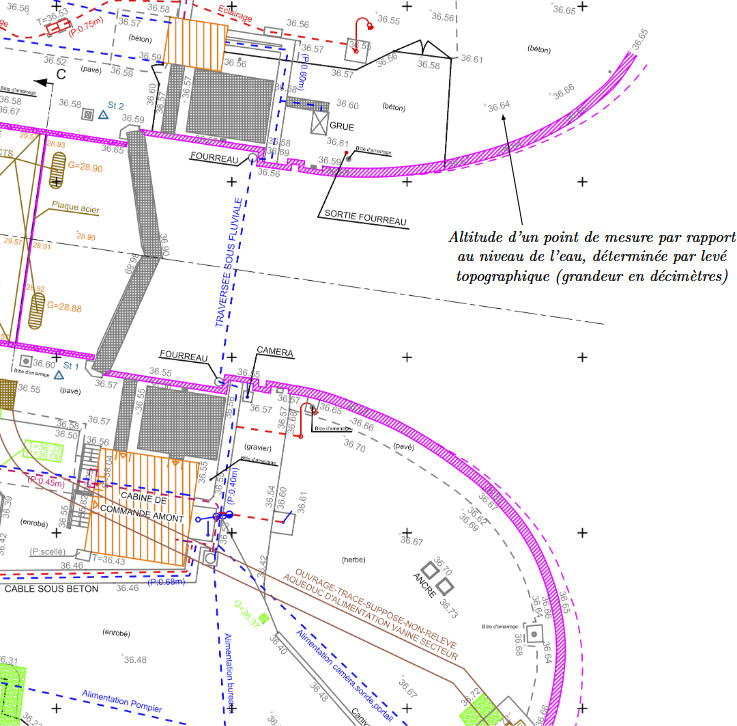
\includegraphics[width=.75\linewidth]{ccs_mp_2017_fig_01.jpg}
\caption{Extrait d’un levé topographique de l’écluse de Saint-Maur-des-Fossés (Val de Marne), réalisé par le bureau d’études topographiques Aérotopo pour le réaménagement des zones techniques \label{CCS_MP_2017:fig_01}}
\end{figure}

La réalisation de levés topographiques sur de vastes chantiers a conduit au développement de systèmes de plus
en plus précis et pouvant réaliser plusieurs mesures successives après une seule prise d’origine.

Les mesures topographiques peuvent être réalisées au moyen de trois systèmes optiques, qui déterminent tous les coordonnées d'un point par rapport à un repère de référence, mais avec des niveaux de précision différents :

\begin{itemize}
  \item le théodolite permet de réaliser des pointages visuels sur une mire, règle comportant des graduations régulières, positionnée verticalement par un opérateur au niveau du point à mesurer;
  \item le tachéomètre est un théodolite qui dispose d'un système de mesure de la distance via le renvoi d'un faisceau laser par un prisme optique rétro-réfléchissant positionné à l'endroit de mesure ;
  \item la station totale est un tachéomètre doté d'un système de communication et d'acquisition des mesures sans fil, ce qui permet la réalisation de mesures en continu.
\end{itemize}

\begin{obj}
L'objectif de ce sujet est d'étudier les mesures topographiques réalisées par l'ensemble théodolite et mire (partie \ref{CCS_MP_2017:p2}) puis par l'ensemble tachéomètre et prisme optique rétro-réféchissant (partie \ref{CCS_MP_2017:p3}) avant d'analyser l'optimisation de ces mesures en utilisant la station totale LeICA TCRA 1103 (partie \ref{CCS_MP_2017:p4}).
\end{obj}

\subsection{Grandeurs mesurées}
Afin de s'adapter à tous les terrains, l'appareil de mesure est placé sur un plateau orientable, lui-même fixé sur un trépied télescopique. La parfaite verticalité de l'appareil, indispensable à la réalisation de levés topographiques précis, est réglée par des vis micrométriques (figure \ref{CCS_MP_2017:fig_02}). Une direction de référence $\vec{x}_{0}$ est choisie par le géomètre, ce qui permet de complètement définir les références des angles d'azimut $\varphi$ et d'élévation $\theta$.\\
La détermination des valeurs des coordonnées $x, y$ et $z$ d'un point $P$ de l'espace dans le repère $R_{0}\left(O_{0} ; \vec{x}_{0}, \vec{y}_{0}, \vec{z}_{0}\right)$ est obtenue par les mesures de l'angle d'azimut $\varphi$, de l'angle d'élévation $\theta$ et de la distance $D$ entre l'isocentre $O$ de l'appareil (point d'intersection des axes de rotation, confondu avec l'origine $O_{0}$ ) et le point $P$ : voir figure \ref{CCS_MP_2017:fig_02}.\\

\begin{figure}[!h]
\centering
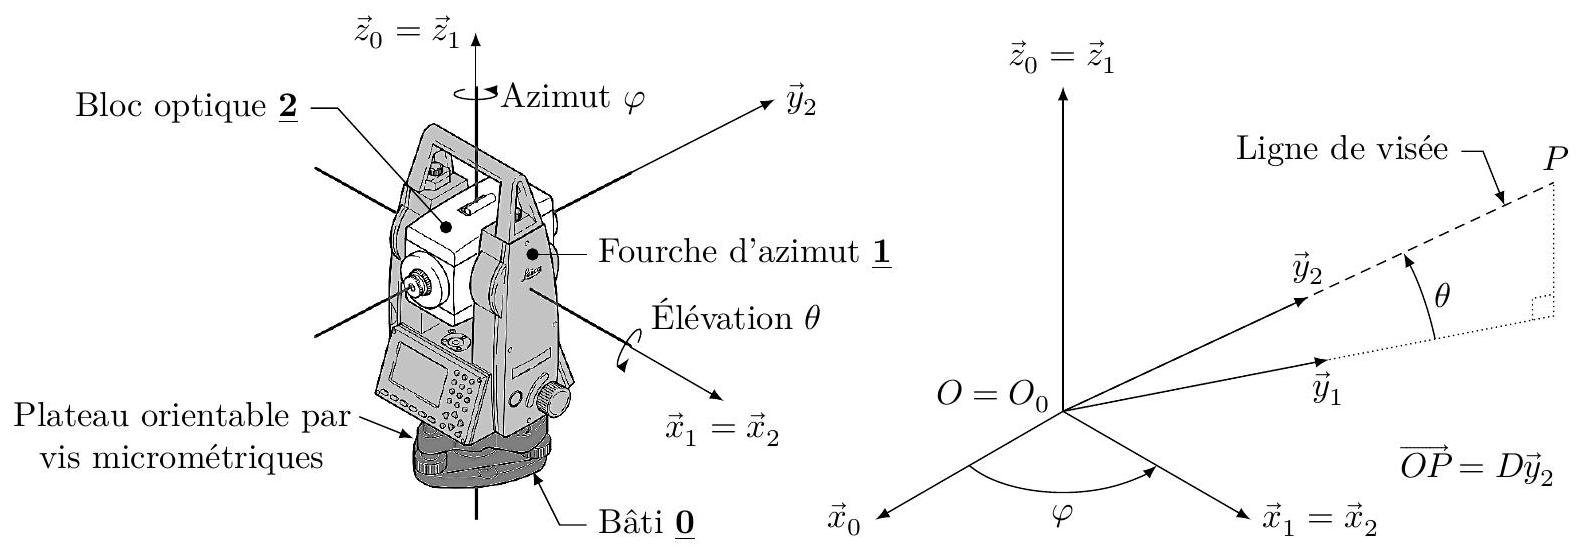
\includegraphics[width=\textwidth]{2024_12_07_51b7f57c7f055c2d8d29g-02}

\caption{Éléments d'un appareil de mesure topographique et grandeurs déterminées \label{CCS_MP_2017:fig_02}}
\end{figure}
%Q 1. 
\question{\label{CCS_MP_2017:q_01}Tracer les figures de changement de base associées aux angles d'azimut $\varphi$ et d'élévation $\theta$ et déterminer les expressions des coordonnées $x, y$ et $z$ de la cible $P$ dans le repère de référence $R_{0}\left(O_{0} ; \vec{x}_{0}, \vec{y}_{0}, \vec{z}_{0}\right)$ en fonction des angles $\varphi$ et $\theta$ et de la distance $D$ entre l'isocentre $O$ de l'appareil et la cible $P$.}

\ifprof
\begin{corrige} ~\\

\begin{center}
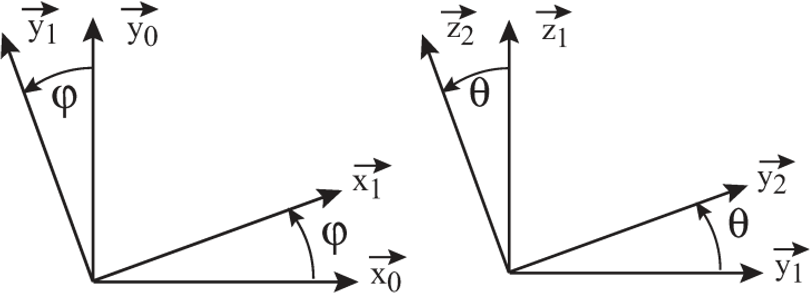
\includegraphics[width=.7\textwidth]{ccs_mp_2017_co_01}
\end{center}
$\vect{OP}=D\vy{2} = \begin{pmatrix} 0 \\ D \cos \theta \\ D \sin \theta \end{pmatrix}_{\mathcal{B}_{1}}$
$= \begin{pmatrix} - D \cos \theta \sin \varphi \\ D \cos \theta \cos \varphi \\ D \sin \theta \end{pmatrix}_{\mathcal{B}_{0}}$.

\end{corrige}
\else
\fi

